%% thesis.tex 2014/04/11
%
% Based on sample files of unknown authorship.
%
% The Current Maintainer of this work is Paul Vojta.

\documentclass[hidelinks]{ucbthesis}
%\usepackage{biblatex}

% To compile this file, run "latex thesis", then "biber thesis"
% (or "bibtex thesis", if the output from latex asks for that instead),
% and then "latex thesis" (without the quotes in each case).

% Double spacing, if you want it.  Do not use for the final copy.
% \def\dsp{\def\baselinestretch{2.0}\large\normalsize}
% \dsp

% If the Grad. Division insists that the first paragraph of a section
% be indented (like the others), then include this line:
% \usepackage{indentfirst}

\setsecnumdepth{subsection} % number sections
\maxtocdepth{subsection}

% Define packages
\usepackage{hyperref, url} 
\usepackage{graphicx,amsfonts,psfrag,layout,subcaption,array,longtable,lscape,booktabs,dcolumn,amsmath,amssymb,amssymb,amsthm,setspace,epigraph,chronology,color,colortbl,wasysym,diagbox,colortbl,authblk,commath,upgreek,natbib}
\usepackage[]{graphicx}\usepackage[]{color}

% Caption keys
\usepackage{mathtools,tikz,caption}
\captionsetup{labelfont=sc,labelsep=period}
\DeclareRobustCommand\sampleline[1]{%
	\tikz\draw[#1] (0,0) (0,\the\dimexpr\fontdimen22\textfont2\relax)
	-- (2em,\the\dimexpr\fontdimen22\textfont2\relax);%
}

\usetikzlibrary{plotmarks}
\usetikzlibrary{automata, positioning}

% Wes Anderson colors

\usepackage{xcolor}

\definecolor{Darjeeling11}{HTML}{FF0000}
\definecolor{Darjeeling15}{HTML}{5BBCD6}

% New footnote characters
\usepackage{footmisc}
\DefineFNsymbols{mySymbols}{{\ensuremath\dagger}{\ensuremath\ddagger}\S\P
	*{**}{\ensuremath{\dagger\dagger}}{\ensuremath{\ddagger\ddagger}}}
\setfnsymbol{mySymbols}

%Rm thanks dagger
\renewcommand\footnotemark{}
%\renewcommand\footnoterule{}

% New tabular environment
\usepackage{tabularx}
\newcolumntype{Y}{>{\raggedleft\arraybackslash}X}% raggedleft column X

% Define appendix 
\renewcommand*\appendixpagename{Appendix}
\renewcommand*\appendixtocname{Appendix}

% Position floats
\renewcommand{\textfraction}{0.05}
\renewcommand{\topfraction}{0.95}
\renewcommand{\bottomfraction}{0.95}
\renewcommand{\floatpagefraction}{0.35}
\setcounter{totalnumber}{5}

% Colors for highlighting tables
\definecolor{Gray}{gray}{0.9}

% Different font in captions
\newcommand{\captionfonts}{\normalsize}

\makeatletter  % Allow the use of @ in command names
\long\def\@makecaption#1#2{%
	\vskip\abovecaptionskip
	\sbox\@tempboxa{{\captionfonts #1: #2}}%
	\ifdim \wd\@tempboxa >\hsize
	{\captionfonts #1: #2\par}
	\else
	\hbox to\hsize{\hfil\box\@tempboxa\hfil}%
	\fi
	\vskip\belowcaptionskip}
%\makeatother   % Cancel the effect of \makeatletter

% Macros
\newcommand{\Adv}{{\mathbf{Adv}}}       
\newcommand{\prp}{{\mathrm{prp}}}                  % How to define new commands 
\newcommand{\calK}{{\cal K}}
\newcommand{\outputs}{{\Rightarrow}}                
\newcommand{\getsr}{{\:\stackrel{{\scriptscriptstyle\hspace{0.2em}\$}}{\leftarrow}\:}}
\newcommand{\andthen}{{\::\;\;}}    %  \: \; for thinspace, medspace, thickspace
\newcommand{\Rand}[1]{{\mathrm{Rand}[{#1}]}}       % A command with one argument
\newcommand{\Perm}[1]{{\mathrm{Perm}[{#1}]}}       
\newcommand{\Randd}[2]{{\mathrm{Rand}[{#1},{#2}]}} % and with two arguments
\newcommand{\E}{\mathrm{E}}
\newcommand{\Var}{\mathrm{Var}}
\newcommand{\Cov}{\mathrm{Cov}}
\DeclareMathOperator*{\plim}{plim}
\newcommand\independent{\protect\mathpalette{\protect\independenT}{\perp}}
\def\independenT#1#2{\mathrel{\rlap{$#1#2$}\mkern2mu{#1#2}}}
\newcommand{\possessivecite}[1]{\citeauthor{#1}'s (\citeyear{#1})} 

\newtheorem{theorem}{Jibberish}

\hyphenation{mar-gin-al-ia}
\hyphenation{bra-va-do}

\begin{document}

% Declarations for Front Matter

\title{Essays on the Political Economy of the American Frontier}
\author{Jason V Poulos}
\degreesemester{Spring}
\degreeyear{2019}
\degree{Doctor of Philosophy}
\chair{Professor Sean Gailmard}
\othermembers{Assistant Professor Joshua Blumenstock \\
  Professor Eric Schickler\\
Professor Jasjeet Sekhon}
\numberofmembers{4}
% Previous degrees are no longer to be listed on the title page.
% \prevdegrees{B.A. (University of Northern South Dakota at Hoople) 1978 \\
%   M.S. (Ed's School of Quantum Mechanics and Muffler Repair) 1989}
\field{Political Science}
% Designated Emphasis -- this is optional, and rare
 \emphasis{Computational and Data Science and Engineering}
% This is optional, and rare
% \jointinstitution{University of Western Maryland}
% This is optional
\campus{Berkeley}

% For a masters thesis, replace the above \documentclass line with
% \documentclass[masters]{ucbthesis}
% This affects the title and approval pages, which by default calls this
% document a "dissertation", not a "thesis".

\maketitle
% Delete (or comment out) the \approvalpage line for the final version.
%\approvalpage
\copyrightpage

% (This file is included by thesis.tex; you do not latex it by itself.)

\begin{abstract}

% The text of the abstract goes here.  If you need to use a \section
% command you will need to use \section*, \subsection*, etc. so that
% you don't get any numbering.  You probably won't be using any of
% these commands in the abstract anyway.

This dissertation argues that early land reforms had consequential long-run impacts on the development of the American state. The state-building role of land reform, frequently discussed in the context of comparative political economy, is often overlooked in the study of American political development. I provide evidence that mid-nineteenth century homestead acts had significant long-run impacts that can help explain contemporary differences in state capacity. I find that homestead policy --- or the homestead entries authorized by homestead policy --- had significant and negative effects on the size of state governments lasting a century after passage of the 1862 Homestead Act. This finding implies that in the absence of homestead policy, the average size of frontier state governments would have exceeded the average size of governments in states that were not directly affected by the policy. Potential causal mechanisms include land inequality, which I show to be positively correlated with state capacity, especially at higher levels of inequality. This empirical relationship is consistent with median voter theories of inequality and redistribution that assume parity in the political influence of voters. 

The dissertation contributes to a new generation of data-driven machine learning methods for estimating causal impacts of policy interventions on panel data. Machine learning approaches are capable of automatically choosing appropriate predictors without relying on pre-intervention covariates, limiting the `researcher degrees of freedom' that arise from model specification choices. The proposed method based on recurrent neural networks can learn nonconvex combinations of predictors, are specifically structured for sequential data, and outperform regression-based estimators in high-dimensional data settings when the number of pre-intervention periods exceeds the number of predictors. The dissertation also introduces a matrix completion method for the problem of counterfactual prediction. The matrix completion method is adaptable to settings with staggered treatment adoption and outperforms RNN-based estimators and other regression-based estimators in small-dimensional data settings.
\end{abstract}


\begin{frontmatter}

\begin{dedication}
\null\vfil
\null\hfil
For Mom
\null\hfil
\vfil\null
\end{dedication}

% You can delete the \clearpage lines if you don't want these to start on
% separate pages.

\tableofcontents
%\clearpage
%\listoffigures
%\clearpage
%\listoftables

\begin{acknowledgements}
	
I thank my advisor, Sean Gailmard, for urging me to think more creatively and to pursue outsize research questions. And for reminding me that I'm not my own harshest critic.\\

I acknowledge support of the National Science Foundation Graduate Research Fellowship (DGE 1106400). Parts of this dissertation used the computer resources of Stampede2 at the Texas Advanced Computing Center under an Extreme Science and Engineering Discovery Environment startup allocation (TG-SES180010) and a Titan Xp GPU donated by the NVIDIA Corporation.
\end{acknowledgements}

\end{frontmatter}

%\pagestyle{headings}

%\part{First Part}
\chapter{Introduction}

This dissertation argues that early land reforms had consequential long-run impacts on the development of the American state. The state-building role of land reform, which includes policies to decentralize public land, is frequently discussed in the context of comparative political economy. Several scholars of American Political Development (APD) have studied the implications of land policies designed to open up the western frontier on the developmental trajectory of the U.S. \citep[e.g.,][]{bensel1990,frymer2014rush}; however, this dissertation is the first to quantify how land policies shaped the developmental trajectory of the American political economy.

In the existing APD literature, substantial attention is paid to state-building with respect to the centralization of national power.  For instance, APD scholars trace the expansion of federal bureaucratic capacity through the merit-based federal civil service system installed in the aftermath of the American Civil War \citep{skowronek1982building,bensel1990,carpenter2001}. The American state, however, is organized horizontally and authority is often delegated downward to sub-national units of government. As \citet{novak2008myth} writes, ``trying to gauge the power of the American state or the reach of American public policy by looking simply at the national center or the federal bureaucracy is to miss where much of the action is --- on the local and state levels." How did public land laws shape the development of state governments?

This dissertation also contributes to the comparative politics literature concerned with land reform and state-building  \citep[e.g.,][]{albertus2015autocracy, murtazashvili2016does}. Land reform refers to policies designed to establish or redefine property institutions to increase land tenure, and includes policies such as land redistribution, land titling, and decentralization of public land. 

The essays included in this dissertation explore the consequences to two different mechanisms of public land decentralization in the 19th century U.S.: land lotteries and homestead policies. The latter offered a free land grant to citizens willing to build on an improve a plot of land of predetermined size for a number of years; land lotteries involved the random allocation of the right to file a land grant, without a homesteading requirement. Both were designed to rapidly populate the frontier with mostly white settlers, thereby reducing the costs of defending unsecured territory for a otherwise constrained national and sub-national governments \citep{frymer2014rush}.

\section{Land reform, inequality and state capacity}

Land reform is an important tool of state-building, which is broadly defined as efforts designed to strengthen weak nation-states states through political and economic reforms. It is generally argued in the state-building literature that greater economic power of the ruling class reduces investment in state capacity. State capacity refers not only to the ability to raise revenue, but also the state’s ability to implement policies such as public education through redistributive spending \citep{besley2010state}. The canonical model of \citet{meltzer1981rational} predicts a positive relationship between inequality and redistribution because greater inequality implies the median voter is poorer than the average voter, which in turn increases demand for redistribution in majority-rule elections. 

The canonical model assumes parity in the political influence of voters. However, economic differences in political influence can arise from the comparative advantage of economic elites in solving collective action problems and benefitting from political intervention \citep{acemoglu2008persistence}. Elites have higher education attainment and earnings abilities \citep{bourguignon2000oligarchy}, and their resource advantage and common interests enable them work toward similar policy goals \citep{winters2009}. 

Models that allow for differences in political influence across economic groups yield a nonlinearity in the relationship between inequality and redistribution. In \possessivecite{benabou2000unequal} model, for instance, the pivotal voter is wealthier than the median and has the power to block redistribution as inequality increases. But when inequality is too high, the poor can impose redistribution on elites through `universal' majority voting \citep{perotti1993political,saint1993education}. In \possessivecite{besley2009origins} framework, greater economic power of the ruling class reduces investment in state capacity. 

\citet{galor2009inequality} propose a model where wealthy landowners block education reforms because education favors industrial labor productivity at the expense of the agricultural sector. Their model implies education reforms will not occur where land is abundant and unequally distributed, and thereby delays the transition from an agricultural to an industrial economy. However, land reforms that sufficiently reduce land inequality diminishes the economic incentives of landowners to block education reforms. 
%
%\citet{albertus2015autocracy} theorizes that the successful implementation of land reform requires sufficient administrative capacity, low institutional constraints, and a coalitional split between landowners and the ruling class that provides the ruling class with the incentive to pursue land reform. 

\subsection{``Hollowing out'' tax institutions}
	
Landed elites might choose an inefficient organization of the state in order to create inefficiencies in tax collection \citep{acemoglu2011emergence} or ``hollow-out'' tax institutions in order to constrain the state's ability to tax in the future \citep{suryanarayan2017hollowing}. Inequality in this context can be thought of as a proxy for the amount of \emph{de facto} political influence elites have to block reforms and limit the capacity of the state \citep{acemoglu2008persistence}.

\citet{mares2015non} argue that higher levels of land inequality increases the likelihood of adopting new taxes in order to give the landed elite the ability to design a tax structure that shifts the tax burden from the agricultural sector to the manufacturing sector. The authors show empirically that countries with high levels of land inequality are more likely to adopt the income tax.  Consistent with the findings of \citet{mares2015non}, I show that land inequality is positively related to state capacity, especially at higher levels of inequality. 

This finding is in contrast to several empirical studies that establish a negative relationship between land inequality and state capacity in the context of taxes, revenues, and public school spending at the county-level in 1890 and 1930. These studies are based on analyses over shorter time periods. \citet{ramcharan2010inequality}, for instance, finds an inverse relationship between land inequality and county-level property tax revenues in 1890. The authors find that the negative relationship is especially large in rural counties, where landownership tends to be more concentrated. \citet{vollrath2013inequality} establish a negative relationship between land inequality and local property tax revenues in 1890 in northern rural counties, but not in southern rural counties. 

\section{Culture and migration to the frontier}

It is commonly believed in the political economy literature that state capacity in general is easier to raise in more ethnically or culturally homogeneous societies \citep{besley2010state}. It has also long been viewed in by sociologists \citep{meyer1979public} and more recently, political economists \citep{alesina2013nation,bandiera2018nation}, that the rise of public schooling in the U.S. during the 19th century can be explained as a nation-building policy enacted primarily by state governments, which were the most active level of government in terms of public goods provision from 1790 to the 1840s \citep{wallis2000american}. \citet{bandiera2018nation}, for instance, argues that states adopted compulsory schooling laws as a nation-building tool to instill civic values to the millions of foreign migrants who arrived to the country between 1850 and 1914, during the `Age of Mass Migration.' 

During this time period, the frontier attracted foreign migrants along with workers from eastern U.S. cities, many of whom were the lower end of the skill distribution. \citet{bazzi2017frontier} find evidence that frontier settlers were disproportionately illiterate and foreign-born. The negative selection of westward migrants during this period is consistent with theory of the frontier as a `safety valve' for relieving congested urban labor markets in eastern states \citep{turner1956significance, ferrie1997migration}.

Beside the negative selection in terms of labor market skill, \citet{bazzi2017frontier} argue that the frontier attracted individualists who would be able to thrive in the harsh conditions characterizing the frontier experience; e.g., the social isolation due to low population density on the frontier. The authors find that counties with longer historical frontier experience exhibit lower contemporary property tax rates, and their citizens are more opposed to taxation and redistribution. 

\section{Land monopolization and rent-seeking on the frontier} 

A competing argument emerges from the dissertation that early land reform in the American case increased the economic power of elites by enabling speculators, railroad companies, and other corporations to scoop up huge swaths of valuable land and then act as passive rentiers.  

The U.S. frontier experienced a large-scale transformation of hundreds of millions of public frontier land into private property beginning with the passage of the Land Act of 1820, which permitted the direct sale of public land to private individuals of 80 acres or more for at least \$1.25 an acre, and accelerating after the passage of the homestead acts. About 150 million acres of public land, or about 7\% of the total area of frontier states, had already been sold by the time of the passage of the Homestead Act (HSA) of 1862.\footnote{Source: author's estimates using land patent data described in Section~\ref{state-capacity}.} By the turn of the twentieth century, 250 million acres (11\% of total land area) had been sold, while 100 million acres (4\% of total land area) had been claimed by homestead. In the South, about 50 million acres of public land, or about 31\% of the states' total acreage, had already been sold by before the passage of the Southern Homestead Act of 1866. A substantial rise in the number and total acreage, respectively, of homestead entries in the South and West occurred after the 1889 cash-entry restriction imposed by the U.S. Congress.

The large-scale transfer of public land to railroad companies may have accelerated the increase in frontier land inequality. Land near railroad tracks were often high quality and railroad companies sold excess land to speculators \citep{murtazashvili2013political}. Railroad companies were granted nearly 130 million acres of land between 1862 and 1871 by federal and state governments. About 20\% of the public domain was granted to states or sold or granted to railroads or other corporations, which is comparable to the amount of land granted or sold to homesteaders \citep{shanks2005homestead}.

Speculators and railroad companies worked together to secure state, county, and municipal grants for local railroads. In \possessivecite{gates1939land} study of Indiana counties, for example, speculators fought county governments subsidizing railroads --- despite possibly benefiting from the lines --- and the speculators' land reduced the tax base of the area, so that counties could not sell bonds to finance railroad subsidies. 

\section{``What the railroad will bring us''} 

Frontier states prioritized spending on banking and transportation projects in competition with each other to raise land values and attract more settlers \citep{sylla1998anatomy}. The promise of increasing land values and future tax revenues led frontier states to sharply increase borrowing in the mid-1830s by selling long-term bonds to finance transportation and banking investments. Frontier states in the Northwest (e.g., Illinois, Indiana, and Michigan) borrowed to invest in canals and railroads, while those in the South (e.g, Arkansas, Florida, and Mississippi) borrowed in order to charter state banks. Indiana, for instance, passed the Mammoth Internal Improvement Act in 1836 that added \$10 million in debt spending for transportation projects such as the Wabash and Erie Canal. The state also changed its property tax structure from a flat tax on land to an \emph{ad valorem} tax on all wealth in order to capture the expected increase in land values that would result from the projects \citep{wallis2004sovereign}. The Panic of 1837 decreased land values and put a hole in the state's tax revenue, causing the state to default on its debt and interest obligations.

Because railroads expanded commerce by making it cheaper to trade, railroad access is theoretically expected to increase returns to farm land, and in turn increase the property tax base. \citet{donaldson2016railroads}, for instance, find that average farm values increased substantially as the railroad network expanded from 1870 to 1890, and estimate that the absence of railroads would have decreased farm land values by 60\%. \citet{atack2011impact} attribute two-thirds of the increase in improved farm acreage in Midwestern states to the expansion of railroad access in the decade prior to the Civil War. As evidence that railroad access increases the property tax base through higher land values, \citet{atack2012impact} find school attendance rates increased in counties that gained access to the rail network between 1850 and 1860. 

\section{Counterfactual history}

Inferring causal relationships is a fundamental problem in history and the social sciences. The problem of causal inference is usually framed in terms of counterfactuals: outcomes that would have been observed had the path of history diverged \citep{lewis2013counterfactuals,pearl2009causality,imbens2015causal}. Historians frequently pose counterfactuals in terms of speculating about the `might-have-beens' of history, as it is put by  \citet{elster1978logic}:

\begin{quote}
``In a non-experimental and non-comparative discipline one can hardly discuss the
relative importance of causes without engaging in some kind of thought experiment where one removes successively and separately each of the causes in
question and evaluates what difference the absence of this cause would have
made to the phenomenon in question. Some historians have come to recognize,
therefore, that they have been talking counterfactually all the time without
recognizing it.''
\end{quote}

This dissertation focuses on counterfactual questions in observational studies, where interventions and outcomes have already been recorded. In observational studies, interventions are not randomly assigned and thus there is no ``reasoned basis for inference'' for evaluating counterfactuals, according to Fisherian view of causal inference \citep{fisher1935}. This absence of randomization has not prevented political scientists from reasoning about counterfactuals in comparative case studies \citep{fearon1991counterfactuals, tetlock1996counterfactual,abadie2010synthetic,abadie2015comparative}.% Economic historians have evaluated counterfactual questions such as, ``What would the U.S. economy have been like in 1890 had there been no railroads?'' using a ``social saving" methodology \citep{fogel1964railroads, donaldson2016railroads} or general equilibrium models \citep{williamson2008late}.

\section{Sample selection bias and covariate shift}
The problem of counterfactual analysis in observational studies is inevitably confronted with sample selection bias \citep{heckman1979sample} which arises because the units choose whether they are exposed to treatment, or because the researcher makes nonrandom sample selection decisions. In either case, inferences on observed samples are biased because they differ from what we would infer on random samples from the population. 

The observational study in Chapter \ref{ga-lottery} makes the case that bias due to self-selection is ignorable because the treatment in the study -- winning land in the first two Georgia land lotteries --- was perfectly randomized by the state of Georgia; i.e., it is a true ``natural experiment.'' In Chapters \ref{land-reform} and \ref{rnns-causal}, it is acknowledged that treatment --- exposure to homestead policy or homestead entries authorized by those policies --- is not randomly assigned and units have selected into treatment. Both of these studies approach the problem of causal inference by counterfactual prediction via machine learning methods. The machine learning methods predict counterfactual outcomes of the treated units, which are then compared to the observed outcomes for estimating casual effects. These methods are data-driven, in that they do not require domain knowledge or pre-intervention covariates to generate counterfactual outcomes.  

In machine learning terms, the sample selection bias problem occurs when test set data are drawn from a true distribution and training data are drawn from a biased distribution, where the support of biased distribution is included in that of the true distribution \citep{cortes2008sample}. The sample selection bias problem is a special case of the covariate shift problem, when the distributions of training and test sets differ \citep{bickel2007discriminative}. 

The problem of causal inference by counterfactual prediction assumes that the training set (i.e., control unit observations) and test set (i.e., treated unit observations) are drawn from the same distribution and therefore, requires inference on a different distribution than training set. The approach described in Chapter \ref{rnns-causal} reweights the training loss function by the propensity score \citep{rosenbaum1983central}.\footnote{Note that the propensity score reweighting of the training loss can also be used to correct for the fact that treatment propensity increases over time in staggered treatment adoption settings, such as in Chapter \ref{land-reform}.} This correction technique, along with other regularization approaches, prevent the model from learning an overreliance on certain control units or time periods when generalizing from the factual to counterfactual domains \citep{johansson2016learning}.
	
\section{Overview}

The dissertation is comprised of the following three essays on the political economy of the American frontier. 

\subsection{State-Building through Public Land Disposal? An Application of Matrix Completion for Counterfactual Prediction}
The essay applies a matrix completion method to predict the counterfactual time-series of frontier state capacity had there been no homestead acts. Causal estimates signify that homestead policies had significant and long-lasting negative impacts on state government expenditure and revenue that lasted a century following their implementation. These results are similar to difference-in-difference (DID) estimates that exploit variation in the timing and intensity of homestead entries aggregated from 1.46 million individual land patent records.

The direction of these estimates align with the view that homestead policies were exploited by land speculators and natural resource companies and that the rents from public land were appropriated by the private sector. I explore land inequality as a possible causal mechanism underlying the relationship between land reform and state capacity, and provide evidence of a positive relationship between land inequality and state government finances and that the slope of correlation increases at higher levels of inequality. I also present DID estimates that reveal per-capita homesteads significantly lowered land inequality in frontier states. The negligible magnitude of the effect suggests that the homesteads did not sufficiently lower land inequality on the frontier, which can explain the negative impacts on state capacity. 

This essay makes a methodological contribution in applying matrix completion for estimating causal impacts of policy interventions on panel data. The method can be easily understood within the framework of modern causal inference, is adaptable to settings with staggered treatment adoption, and outperforms several other regression-based estimators in a battery of placebo tests.

\subsection{Land Lotteries, Long-term Wealth, and Political Selection} 
This essay asks whether personal wealth can cause individuals to select into office. This question is important and relevant because wealthy individuals might select into office in order to use their power to protect vested interests rather than advance the interests of their constituents. While several studies have studied the effect of officeholding on wealth accumulation, research on the extent to which personal wealth affects the probability of officeholding is much more limited.

The essay takes advantage of the random assignment of land in Georgia at the beginning of the nineteenth century. This random assignment of land generates a meaningful ex-ante exogenous shock to personal wealth, which is expected to reduce the opportunity costs of holding office and may make it more important for the wealthy to hold office. I find no evidence in support of the hypotheses that wealth increases the probability of running for office or holding office and argue that these null results are informative because the estimated effects are not practically different than zero. The absence of a treatment effect suggests that observed cross-sectional correlations between wealth and officeholding are likely due to selection effects. 

\subsection{RNN-Based Counterfactual Prediction, with an Application to Homestead Policy and Public Schooling}

This essay makes a methodological contribution in proposing a novel alternative to the SCM for estimating the effect of a policy intervention on an outcome over time. The proposed method based on recurrent neural networks (RNNs) is less susceptible to $p$-hacking because it does not require the researcher to choose predictors or pre-intervention covariates to construct the synthetic control. Moreover, RNNs do not assume a functional form, can learn nonconvex combinations of control units, and are specifically structured to exploit temporal dependencies in sequential data.

The RNN-based estimators require sufficient pre-period observations in order to learn an informative representation of the control units, and consequently perform comparatively worse than the SCM on small-dimensional datasets such as those featured in the original synthetic control papers. The RNN-based methods outperform the SCM in high-dimensional data settings when the number of pre-intervention time periods exceeds the number of control units.

In the empirical application, I estimate the causal impacts of the HSA on state government education spending. I find that homestead policy had positive long-run impacts on public education spending, although the impacts are not statistically significant when averaging across the entire post-intervention period. Time-specific causal estimates suggest that the HSA had positive and significant impacts on state government education spending fifty years after the first homestead entry in 1869. The estimated increase in education spending attributable to homestead policy translates to about 3\% of the total school expenditures per-capita in 1929. % Introduction and background to the general topic area.
\include{chap1} % land-reform
\chapter{Land Decentralization by Lottery} \label{land-lotteries}

A history of land lotteries as they relate to land reform on the frontier... 

	 % transistion into ga-lottery
\chapter[Land Lotteries, Long-term Wealth, and Political Selection]{Land Lotteries, Long-term Wealth, and Political Selection\footnote{This paper is previously published \citep{poulos2019land}.}}\label{ga-lottery}

\begin{quote}  
	\textbf{Summary:} Does personal wealth cause individuals to select into public office? This study exploits the 1805 and 1807 Georgia land lotteries to investigate the hypothesis that wealth increases political power. Most eligible males participated in the lotteries and more than one-in-ten participants won a land prize worth over half of median property wealth. I find no evidence that lottery wealth increases the likelihood of officeholding or running for office, and argue that those null findings are informative because the estimates are not practically different from zero. The absence of a treatment effect implies that commonly observed cross-sectional correlations between personal wealth and officeholding are likely explained by selection effects.
\end{quote}

\clearpage

\section{Introduction}

\noindent
A problem in representative democracies is that elected officials might use their power to defend vested interests rather than advance the interests of their constituents. Personal wealth is expected to reduce the opportunity costs of holding public office and also may make it more important for wealthy citizens to seek elective or appointive positions. While several studies have examined the effect of officeholding on wealth accumulation  \citep[e.g.,][]{eggers2009,querubin2013,truex2013}, research on the extent to which wealth affects officeholding is more limited. 

Natural experiments that exploit exogenous variation in personal wealth can be used to identify wealth's causal effects on officeholding. State-run lotteries that randomly distribute land titles to individuals satisfy that objective because winning a land title represents an exogenous shock to personal wealth. \citet{rossi2014}, for instance, exploits the random allocation of land in $16^{th}$ century Argentina to identify the causal relationship between wealth and subsequent political power. Wealth is proxied by the distance of randomly allocated land from the City of Buenos Aires, where land closer to the city is more valuable and political power is represented as a binary variable indicating whether heads of household or their relatives held a position in city government. Rossi finds that an increase of one standard deviation in the distance of the land to the city reduces the likelihood of political power by about 12\%.\footnote{The linear model used to obtain the estimate assumes that distance of the land to the city is uncorrelated with unobserved individual-level predictors of political labor supply, such as the opportunity costs associated with holding office.}

The present study uses the first two Georgia land lotteries as natural experiments to investigate the hypothesis that personal wealth increases subsequent political power. The 1805 lottery was the first public land lottery in U.S. history, only to be replicated in 1807 and six later Georgia lotteries.\footnote{The six later Georgia lotteries were held in 1820, 1821, 1827, 1832, 1832 (``Gold Lottery''), and 1833 (``Fractions Lottery'').} The state distributed more than one million acres of land in the 1805 lottery, two million acres in the 1807 lottery, and 23 million acres in all eight lotteries \citep{cadle1991}. A sizable majority of eligible adult white males participated in the lotteries, and about one-in-ten won land prizes with an estimated mean value of least \$800, which represents more than half of median property wealth at the time of the lotteries. Since land prizes could readily be sold in a secondary market for public land, the random assignment of land generates an ex-ante exogenous shock to personal wealth. However, I find no evidence in support of the hypotheses that wealth increases the likelihood of officeholding or political candidacy. I argue that those null results are still informative because the estimates are not practically different from zero. 

Did winning the lottery not affect officeholding or candidacy because the magnitude of the windfall --- while large relative to average wealth --- was not sufficient to move the median participant into the slaveholding elite that formed the largest political class in the antebellum South? To determine  whether treatment translates into long-run wealth for lottery winners, I link the participant records to the full-count 1820 Census, which is the earliest census to include a measure of individual wealth: the number of slaves owned. I provide evidence from quantile regression estimates that winning a prize in the 1805 lottery conferred on lottery winners near the median of the wealth distribution a \$171 increase in wealth, with a 95\% confidence interval of [\$18, \$323]. The upper bound of the estimate is enough wealth to satisfy the freehold qualification for running for representative to Georgia's legislature. The estimate is similar in size to \possessivecite{bleakley2013up} estimate that winning a prize in the 1832 Georgia lottery significantly increases 1850 total census wealth (i.e., combined slave and real-estate wealth) by \$200.\footnote{The authors use a sample of 1832 lottery participants linked to the full-count 1850 Census to investigate the effects of lottery prize values on the long-run wealth distribution of lottery winners. Using the same linked sample, \citet{bleakley2016} finds no evidence of a treatment effect on the wealth, literacy, or occupational standing of lottery winners or their descendants.} 

This paper proceeds as follows: Section \ref{theory} provides a theoretical discussion of the channels through which wealth may or may not impact political power; Section \ref{history-ch2} provides some historical background, including details on the development and implementation of the 1805 and 1807 lotteries. Section \ref{data} describes the data and record-linkage procedure, and provides summary statistics on the wealth of officeholders. Section \ref{results} specifies the treatment effect estimator, tests the assumption of random treatment assignment, and provides treatment effect estimates. Section \ref{discussion-ch2} discusses concerns regarding statistical power and the importance of treatment; Section \ref{conclusion} concludes.

\section{Theoretical considerations} \label{theory} 

Through which channel should we expect wealth to influence officeholding, both in general and in the case of the antebellum South? In general, wealth makes it easier to access politics or makes it more important to have political power in order to protect vested interests. Materialist interpretations of oligarchies view personal wealth as a source of political power because it is tightly concentrated among a minority of the population, can be translated into political influence, and accompanies a set of political interests, such as wealth defense \citep{winters2009}. According to that interpretation, wealthy citizens do not need to hold office or explicitly coordinate their political efforts, but instead work toward similar policy goals through political investment or lobbying.

In the case of antebellum Georgia, wealth shocks could have enabled poor citizens to overcome freehold requirements for holding office and attenuate the opportunity costs associated with candidacy and officeholding since the state legislature was not yet professionalized. Citizen-candidate models \citep{osborne1996,besley1997} demonstrate that the number of candidates entering political contests declines with the cost of running, which is modeled both as campaigning cost and the opportunity cost of entering political races. In such models, the set of eligible candidates is the universe of eligible voters. In antebellum Georgia, the former was a proper subset of the latter because many otherwise eligible citizens could not run for office owing to freehold requirements for officeholding.

\citet{corvalan2018political} build on the citizen-candidate model by adding a wealth-based eligibility requirements, which results in ideological distributions differing between eligible candidates and voters. Their model predicts that when the eligibility requirement is high enough to be binding --- i.e., when the eligibility requirement exceeds the median wealth of the constituency --- the key player is the citizen closest to the median within the set of eligible candidates. When the eligibility requirement does not bind, the key player is the constituency median. Eligibility requirements that are not binding can still restrict electoral competition in equilibrium by ruling out the possibility of poorer candidates who prefer higher taxes.

As described in further detail in Section \ref{barriers}, wealth-based eligibility requirements in Georgia were not binding in the sense that they did not exceed the estimated median property wealth at the time of the land lotteries. The lotteries initiated an exogenous shock to the wealth distribution that would have provided poor citizens with the freehold eligibility required to run for the state legislature. In the context of \citet{corvalan2018political}, the exogenous wealth shock resulting from the land lotteries therefore had an  effect on tax policy and electoral competition identical to lessening eligibility restrictions for officeholding: the decisive citizen becomes less wealthy and more favorable to income redistribution, potentially opening the door for ``leftist'' candidates.  

Wealth shocks resulting from the lotteries likewise may have lowered the opportunity costs associated with officeholding, especially considering that Georgia's legislature was not professionalized at the time. State legislatures that are not professionalized tend to be dominated by proprietors rather than wage and salary earners, who face higher opportunity costs of serving \citep{fiorina1994,fiorina1999}. Studies of legislative careers and strategic retirements generally find that nonpolitical wealth and tenure in office are inversely related. \citet{hall1995}, for instance, find that a significant number of U.S. Representatives decided to postpone retirement in 1990 in order to take advantage of a pension windfall enacted by the outgoing Congress. \citet{groseclose1994} estimates that the opportunity cost of remaining in office accounts for more than a third of retirements in 1992, which was the final year in which Members of Congress could transform campaign funds into personal wealth.\footnote{Relatedly, \citet{milyo1999electoral} find that incumbent wealth is orthogonal to electoral success in the 1992 House elections.}

\section{Historical background} \label{history-ch2} 

Inequality in political represenation was prevalent throughout the antebellum South. For example, \citet{helper1860} rails against the ``slave-driving oligarchy'' which dominated political offices then: 
%
	\begin{quotation}The magistrates in the villages, the constables in the districts, the commissioners of the towns, the mayors of the cities, the sheriffs of the counties, the judges of the various courts, the members of the legislatures, the governors of the States, the representatives and senators in Congress --- are all slaveholders....There is no legislation except for the benefit of slavery and slaveholders.
	\end{quotation}  
%
The slaveholders' dilemma was to secure political dominance amid universal white male suffrage. The 1798 Georgia constitution, which was in effect for the entirety of the antebellum period, extended rights to elect members of the legislature to adult white males. Propertyless whites were discouraged from voting on account of a poll tax that the legislature maintained during the antebellum period. Slaveholder candidates, however, often paid the poll taxes of poor whites in exchange for political support \citep{meyers2012}. Slaveholding cotton planters found allies in members of the clerical and the professional classes, who often owned a few slaves for personal service, and that alliance created a class of ``social retainers'' who defended the interests of slaveholding planters \citep{simons1912}. Echoing the U.S. Constitution of 1787, the three-fifths clause in the 1798 Georgia constitution counted slaves as three-fifths of a person for the purpose of representation in the legislature and thus fortified the slaveholders' control of the legislature \citep{coulter1960}.

\subsection{Barriers to officeholding} \label{barriers}

The 1798 Georgia constitution also tied officeholding eligibility to land and property values. Beyond age and residency requirements, candidates for state representative were required to own freehold estates worth \$250 or possess \$500 of taxable property within their constituencies. The eligibility requirements for state senator were double those amounts. Qualifications for governor, an office opened to direct elections in 1824, included owning at least 500 acres of land within the state and other property to the value of \$4,000. Amendments to the constitution removed freehold qualifications for the legislature in 1835 and for governor in 1847. 

In the terminology of \citet{corvalan2018political}, the freehold requirements for serving in the legislature were not binding because the requirements did not exceed the estimated median property wealth at the time of the land lotteries. Drawing a sample from the full-count 1850 Census \citep{ruggles2015} of adult male heads-of-household who were born in Georgia, living in Georgia, and had nonmissing surnames and property values, I estimate that about 13\% of otherwise-eligible citizens had nominal property values below the freehold requirement for state representative and 28\% were barred from running for state senator.

However, winning a land lottery prize enabled otherwise eligible lottery winners who did not satisfy freehold qualifications to hold office in the legislature. Using county-level data from the 1850 Census \citep{haines2004}, I estimate that the mean value of a land prize in either of the first two lotteries exceeded \$800, which represents 55\% of median property wealth at the time of the lotteries.\footnote{Table \ref{counties-tab} provides information on the estimated lot value per county and a description of how the mean land prize values are calculated.}

Georgia's legislature was not professionalized at the time of the lotteries and was mandated by the constitution to meet only once a year.\footnote{The legislature typically met more than once. For example, in 1805 the House and Senate each met about 30 times.} The 1798 constitution provides salaries only for members of the executive branch and judiciary, while \textit{per diem} compensation for legislators was not introduced until the 1877 constitution. The lack of legislative professionalism may have imposed an additional barrier for less wealthy citizens to run for the legislature owing to the opportunity costs associated with holding office.

\subsection{Officeholder wealth}\label{political-class} 

How does the wealth of Georgia's political class compare with the wealth of the general population?  Following the record linkage procedure described in Section \ref{data}, I link the full list of officeholders to the 1820 and 1850 censuses in order to get a sense of where officeholders stand in the distribution of slave wealth and real estate wealth, respectively.\footnote{The match probability averages are close to zero because the model is trained on a different domain; i.e., linking 1807 participants to officeholder records. I drop the prediction threshold to 25\% in order to compensate for lower average match probabilities.} I successfully link 39\% and 66\% of officeholders to the 1820 and 1850 Censuses, respectively. In comparison, \citet{corvalan2018political} report success rates of between 41\% and 68\% when linking the names of state senators from the Carolinas and Virginia to the full-count 1850 Census. 

Table \ref{officeholders-1820-1850} reports basic summary statistics on the wealth-holding of officeholders versus the rest of the sample. Officeholders matched to the 1820 Census hold \$548 more in slave wealth, on average, than the rest of the sample ($p < 0.001$). Similarly, officeholders matched to the 1850 Census hold about \$400 more in real estate wealth, on average, than non-officeholders ($p < 0.001$).

\subsection{The 1805 and 1807 lotteries} \label{lotteries} 

In the wake of public land fraud scandals, Georgia's legislature created a lottery system to distribute 1.3 million acres of newly acquired public land ceded by the Creek tribe. The 1805 lottery carved out three new counties from that land: Baldwin and Wilkinson counties, each divided into five districts, and Wayne county, divided into three districts \citep{clayton1812}. The 1807 lottery extended the boundary between Baldwin and Wilkinson, more than tripling the number of districts within the two counties.  

Free white adult men and orphaned children were eligible for a single draw, while married men with children and widows with children were eligible for two draws in the 1805 lottery. The eligibility rules for the 1807 lottery were similar, with the main exception being that adult unmarried females could participate and 1805 lottery winners were excluded from participation.\footnote{Participants were required to take an oath when ``doubt exist in the minds of the said justices'' regarding the veracity of participants' eligibility. The legislature criminalized making false statements concerning eligibility in the land lotteries. The law specifies that if found guilty in a jury trial, half of the defendant's land went to the informer and the other half is reverted to the state, to be auctioned as land fractions.} Registration for each lottery was voluntary and required a payment of 12.5 cents per draw. I estimate that approximately 85\% of eligible males living in Georgia participated in the 1805 lottery and 70\% of eligible males participated in the 1807 lottery.\footnote{The 1805 calculation was made by taking the proportion of adult male participants over the total white male population aged 16 and over in the 1800 Census. The 1807 calculation subtracts the number of adult male winners in the 1805 lottery from the numerator.} 

Prior to each lottery, a surveyor was appointed by the legislature to map the districts into square lots. During the 1805 lottery, tickets representing each lot were placed in a wooden lottery wheel to be awarded as prizes, along with blank tickets equal in number to the difference between the number of prizes and the number of draws. Two lottery wheels were used in the 1807 drawing: one containing the names of participants, and the other containing lot numbers. Blank tickets in number equal to difference between the number of registered draws and lot prizes were added to the lottery wheel. Tickets from each wheel were drawn simultaneously to form a combined ticket, and the participant won if the combined ticket included a prize. Lottery winners were required to pay \$4 per hundred acres for lots won in the 1805 lottery, or \$6 per hundred acres for lots won in the 1807 lottery, in order to obtain the title on the lot.\footnote{Lottery winners had 12 months following the drawing to claim their prize under law; however, the legislature extended the deadline for claiming prizes on an annual basis until 1815. If lottery winners did not claim their land prior to the deadline, then the lots reverted to the state and sold in a public auction.} 

Winning a prize in the lottery represents a pure wealth shock because no homesteading requirement was imposed and lottery winners could easily sell their grants in a secondary market for public land \citep{weiman1991}. In some cases, lottery winners sold their grants to land speculators, who in turn sold the land to out-of-state settlers \citep{davis1981}. Land speculators often sought out lottery winners who drew particularly valuable lots \citep{cadle1991}.

\section{Data and descriptive statistics} \label{data}

The primary source of data for this study is \possessivecite{graham2004} record of 1805 lottery winners and losers. The 1805 lottery is the only Georgia lottery to have recorded the names of all lottery participants. The records contain information on participants' names, county of registration, lottery draws, and lottery prizes won. Identifying remarks next to the participants' names provide additional information, such as generational suffix (i.e., `Jr.' and `Sr.') and orphan status. Table \ref{summary-table} reports that 15\% of the unrestricted sample of 1805 lottery participants ($N=23,927$) received at least one lottery prize and was registered for 1.65 draws, on average, and 4\% of 1805 lottery winners ($N=3,707$) won two prizes.

I use lottery winner grant records for the 1807 lottery \citep{graham2011} to construct a sample of 1807 lottery winners ($N = 8,822$), in which 14\% of the sample won two prizes. Since the 1807 lottery records do not include information on the number of registered draws, I impute the number of draws by assigning two draws to all participants, except for women and orphans, who are assigned one draw. The mean of the imputed number of draws among 1807 winners, 1.85 draws, is virtually identical to the mean of the actual number of registered draws registered by 1805 winners.

In order to test the hypothesis that wealth increases the probability of officeholding, I link participant names to a historical roster of officeholders published in the \textit{Georgia Official and Statistical Register} \citep{archives1978, archives1990}. The roster includes information on names, jurisdictions, and term dates for all elected and appointed officeholders from the state's colonial period to 1990. I consider officeholders whose first term began in 1805 or 1807 to 1850, inclusive. That decision is based on the fact that the white male life expectancy at age 20 in the early 1800s was approximately 40 years \citep{hacker2010}, the youngest participants who were both eligible for the lottery and public office were 21 years of age and were expected to live 40 additional years. 

I employ a machine learning approach for linking lottery participants to officeholder records. First, I link 1807 lottery winners to officeholders based on an exact match on surname and a phonetic algorithm (i.e., Soundex) code of first name, and then deduplicate the matched records manually. Second, I train an ensemble of algorithmic models on the 1807 records to classify correct matches, using participant characteristics (e.g., the frequency and lengths of surnames) and match characteristics (e.g., the Euclidean distance between participants' county of registration and officeholders' constituency) as features of the model.\footnote{The cross-validated mean squared error on the training set is less than 3\%. Table \ref{ensemble-tab-link} provides information on the record link ensemble's candidate learners, weights, and error estimates.} Lastly, I use the ensemble fit to deduplicate automatically 1805 participant records matched with officeholders on the basis of an exact match on surname and Soundex code of the first name; a prediction threshold of 50\% is adopted to classify correct matches. Thus, the \textit{Officeholder} outcome variable is a binary variable indicating whether the participant is linked to the officeholder records.

As reported in Table \ref{summary-table}, 17\% of adult males who participated in the 1805 lottery are matched to officeholder records successfully, and about one-in-ten of matched participants held office before the drawing of the 1805 lottery. Three-quarters of participants linked to officeholder records first served in the state House, while the rest started their political careers in the state Senate, U.S. House, or other state executive branch offices.

\subsection{Candidacy}

To address the question of whether wealth makes individuals more likely to be candidates for office, I extract candidate names from two election datasets, the first covering all offices from the local level to the federal level from 1787 to 1825 \citep{lampi2012} and the second covering federal offices from 1788 to 1990 \citep{inter1984}. I link participants to candidates who first ran for office between the period of 1805 or 1807 to 1850 using the same deduplication model used for linking participants to officeholder names.\footnote{I lower the prediction threshold to 12.5\% to adjust for candidate match probabilities that average near zero.} The resulting \textit{Candidate} outcome is a binary variable that captures whether participants ran for office. Since the candidate records are more limited in scope compared to the officeholder records, only about 2\% of 1805 and 1807 lottery participants are successfully linked to candidate records, and about a quarter of these matched participants ran for office prior to 1805 or 1807.

\subsection{Future wealth}

Finally, I investigate whether winning a lottery prize increased long-term wealth by linking the participant records to the full-count 1820 Census and estimating the treatment effect on imputed slave wealth. The 1820 Census is the earliest surviving enumeration of Georgia's population and represents all counties except for Franklin, Rabun, and Twiggs counties. The records include information on the name of the head of household and the number of slaves held by gender and age group, which I use to impute slave wealth.\footnote{Access to the full-count data is granted by agreement between UC Berkeley, and the Minnesota Population Center \citep{ruggles2015}. The Minnesota Population Center has collected digitized census data for 1790-1930 microdata collection with contributions from Ancestry.com and FamilySearch.} I match 18\% of 1805 lottery participants and 40\% of 1807 lottery winners to the 1820 Census. The mean slave wealth in the linked samples is between \$1,222 and \$1,971, which is approximates the market value of two male prime-age field hands in Georgia at the time of the lotteries.\footnote{ \citet{phillips1905} estimates the average value of male prime field hands (18-30 years old) in Georgia in 1821 is \$700. I impute slave wealth in 1820 by using the coefficients in Table II of \citet{kotlikoff1979} to adjust this average value according to age group and gender.}

\begin{table}[htbp] 
	\begin{center}
		\caption{Distribution of pretreatment and response variables by sample.\label{summary-table}}   
		\resizebox{0.9\width}{!}{\input{/media/jason/Dropbox/ga-lottery-local/paper-drafts/ga-lottery-manuscript/summary-table}}
	\end{center}
	\footnotesize{Notes: \textit{Treated } is defined as winning at least one prize for the 1805 winners and losers sample, and winning two prizes for the samples restricted to winners. \textit{\# draws} is the number of registered draws. \textit{Candidate} and \textit{Officeholder} indicates whether participants ran for office or held office, respectively. \textit{Slave wealth} (in 1820 dollars) is the imputed slave wealth for participants matched to the 1820 Census.} 
\end{table}

\section{Estimation and results} \label{results} 

I estimate the following linear model:

\begin{equation} 
y_{i,s} =  \text{\# draws}_{i,s} + \delta \, \text{treat}_{i,s} + \epsilon_{i,s}, \label{eq:lm} 
\end{equation} 
\noindent
where $y_{i,s}$ is the candidate or officeholder response or 1820 slave wealth measure for participant $i = \left\{1, ..., N \right\}$ in sample $s$ and $\text{\# draws}_{i,s} \in \{1,2\}$ represents the number of draws registered by each participant. When the sample includes both 1805 winners and losers, $\text{treat}_{i,s}$ is a binary treatment assignment variable that assumes a value of unity for participants who won at least one prize in the 1805 lottery and assumes a zero value for participants who did not win a prize. The coefficient of interest, $\delta$, corresponds to the intention-to-treat (ITT) estimate of the sample average treatment effect. When the sample is limited to winners in either the 1805 or 1807 lotteries, $\text{treat}_{i,s}$ is equal to unity for participants who win two prizes in the lottery and is zero otherwise. In that case, the ITT effect captures the marginal effect of winning a second land prize. 

\subsection{Balance}

The model assumes that treatment assignment is random conditional on the number of registered draws. While that assumption cannot be tested directly, we can verify that treatment assignment with respect to the pretreatment covariates is balanced. Statistically significant treatment effects on pretreatment covariates at the level of $\alpha= 0.05$ indicate imbalance in treatment assignment. 

Fig. \ref{balance-plot} plots the $p$-values corresponding to the treatment effect estimated by estimating Eq. \ref{eq:lm} on each pretreatment covariate summarized in Table \ref{summary-table}. Treatment assignment is balanced across all pretreatment covariates for 1805 lottery winners and losers. When the sample is restricted to 1805 lottery winners, winners registered in Clarke County were more likely to have won two prizes rather than a single prize, controlling for the number of draws ($p=0.02$). However, the difference is not significant when accounting for the multiple comparisons made for the balance tests.\footnote{The significance level for the Bonferroni correction is $\alpha= 0.05/33 = 0.001$.}

In the sample of 1807 lottery winners, winners who ran for office prior to the 1807 lottery were more likely to have won a second prize ($p = 0.01$). Additionally, 1807 lottery winners were more likely to have won a second prize if they also were more likely to be matched to the 1820 Census ($p < 0.01$), have names with generational suffixes ($p < 0.01$), or have more common surnames ($p < 0.01$). Treatment assignment likewise is unbalanced for 1807 winners registered in the counties of Bryan, Clarke, and Lincoln. 

\begin{figure}[htbp]
	\caption{Balance in treatment assignment by lottery sample.\label{balance-plot}}
	\begin{center}
		\includegraphics[width=0.85\linewidth]{/media/jason/Dropbox/ga-lottery-local/paper-drafts/ga-lottery-manuscript/balance-plot.jpeg} 
	\end{center}
	\footnotesize{Notes: \textit{1820 Census Match} is the probability of being linked to the 1820 Census;  \textit{Candidate} and \textit{Officeholder} indicates participants who ran for or held office, respectively, prior to the 1805 lottery. Samples include all lottery participants.}
\end{figure}

\subsection{ITT estimates}

Table \ref{itt-table} presents the ITT treatment effect estimates on each outcome of interest. The confidence intervals for the ITT estimates on officeholding tightly straddle zero for each sample. In the discussion below, I argue that these null results on officeholding are informative because the estimated effects are not practically different from zero. For example, the upper bound of the interval of the treatment effect estimate on \textit{Officeholder} implies that, at most, 1\% of the sample treated group would select into office as a result of receiving treatment. The confidence interval for the estimate is unchanged when estimating the effect on officeholder match probability (Table \ref{officeholding-robust-table}). 

While I find no evidence of a treatment effect on candidacy for the sample of 1805 winners and losers, the point estimates for the samples of 1805 and 1807 winners imply that the marginal effect of winning a second prize in the lottery significantly increases the probability of running for office by 1\% to 2\%. However, those estimates are not robust to using candidate match probability as the outcome variable (Table \ref{candidate-robust-table}). 

Lastly, I find no evidence that winning a prize in the 1805 lottery increased future slave wealth. In the sample of 1807 winners, winning a second prize significantly reduces slave wealth in 1820 by \$163 [-\$256, -\$69]; although, that estimate is not robust to including pretreatment covariates in the regression or weighting slave wealth by the probability of being matched to the 1820 Census (Table \ref{slave-robust-table}).

\begin{table}[htbp] 
	\begin{center}
		\caption{ITT treatment effect estimates.\label{itt-table}}   
		\resizebox{0.9\width}{!}{\input{/media/jason/Dropbox/ga-lottery-local/paper-drafts/ga-lottery-manuscript/itt-table}}
	\end{center}
	\footnotesize{Notes: values in brackets represent 95\% confidence intervals for treatment effect estimates derived from the standard errors of the linear model (Eq. \ref{eq:lm}). Orphans and women are excluded from each sample for candidacy and officeholding outcomes.}
\end{table}

\section{Discussion} \label{discussion-ch2}

In the short-run, treatment enabled lottery winners at the lower-end of the wealth distribution to meet the freehold qualifications for holding office in the state legislature. Still, treatment may be too weak to cause a substantively meaningful increase in the likelihood that lottery winners would select into public office, given how rare an event it is for citizens to become elected officials. I conduct a power analysis by simulation to ensure that the research design allows for the identification of a significant treatment effect. The simulation results imply that if the actual treatment effect size in a hypothetical finite population is 2.1\%, the research design provides an 80\% chance of rejecting the null hypothesis that treated and control participants are equally likely to hold office (Fig. \ref{power-plot-bin}). Since I am unable to reject the null in the sample, it follows that the population effect size is most likely less than 2.1\%, an effect not practically different from zero. 

Is it the case that the null effects for officeholding are driven by the fact that lottery wealth does not translate into larger long-run wealth, but rather increases present consumption? Lottery winners may perceive lottery wealth as a financial windfall and spend the winnings more quickly than earned wealth \citep{doherty2006}. While I find no evidence that winning a prize in the 1805 lottery increased the future wealth of lottery winners, I provide evidence from quantile regression estimates that treatment increased future wealth for 1805 lottery participants near the median of the wealth distribution (Fig. \ref{qreg-plot}). Specifically, I find that treatment confers a \$171 [\$18, \$323] increase in wealth for participants at the median. The upper bound of the confidence interval represents an increase in wealth sufficient to satisfy the freehold qualification for running for state representative. 

While winning a land lottery prize enabled otherwise eligible lottery winners who did not satisfy freehold qualifications to hold office in the legislature, pervasive wealth inequality may have played a role in stifling access to politics in Georgia in the early $19^{th}$ century. In 1850, the top decile of property-owners held over half of the total property wealth in that state.\footnote{The calculation uses a sample of adult male heads of household who were born in Georgia and were living in Georgia at the time of the 1850 Census. The statewide slave wealth Gini coefficient in 1820 is 0.78 and the coefficient for statewide real estate wealth in 1850 is 0.66, both indicating substantial wealth inequality.} It may be difficult in this setting for even the \textit{nouveau riche} to overcome barriers to entry into politics, such as the opportunity costs associated with participating in politics. Further investigations in alternative settings would help determine whether the results of the present study would be different in a context of less wealth inequality. 

\section{Conclusion} \label{conclusion} 

This study exploits the first two land lotteries in U.S. history to estimate the effect of lottery wealth on subsequent political power. Personal wealth is expected to reduce the opportunity costs of holding office and may make it more important for the wealthy to seek and to hold office. In the case of antebellum Georgia, wealth shocks could have enabled poor citizens to overcome freehold officeholding requirements and lower the opportunity costs associated with officeholding since Georgia's legislature was not yet professionalized. I find no evidence in support of the hypotheses that wealth increases the probability of running for or holding office. 

The null findings nevertheless are informative because the estimated effects are not practically different from zero. What is more important, the absence of a treatment effect implies that commonly observed cross-sectional correlations between personal wealth and public officeholding are likely explained by selection effects.  % ga-lottery
\chapter{Counterfactual History} \label{counterfactual-history}

Inferring causal relationships is a fundamental problem in history and the social sciences. The problem of causal inference is usually framed in terms of counterfactuals: outcomes that would have been observed had the path of history diverged \citep{lewis2013counterfactuals,pearl2009causality,imbens2015causal}. Historians frequently pose counterfactuals in terms of speculating about the `might-have-beens' of history, as it is put by  \citet{elster1978logic}:

\begin{quote}
``In a non-experimental and non-comparative discipline one can hardly discuss the
relative importance of causes without engaging in some kind of thought experiment where one removes successively and separately each of the causes in
question and evaluates what difference the absence of this cause would have
made to the phenomenon in question. Some historians have come to recognize,
therefore, that they have been talking counterfactually all the time without
recognizing it.''
\end{quote}

This dissertation focuses on counterfactual questions in observational studies, where interventions and outcomes have already been recorded. In observational studies, interventions are not randomly assigned and thus there is no ``reasoned basis for inference'' for evaluating counterfactuals, according to Fisherian view of causal inference \citep{fisher1935}. This absence of randomization has not prevented political scientists from reasoning about counterfactuals in comparative case studies \citep{fearon1991counterfactuals, tetlock1996counterfactual,abadie2010synthetic,abadie2015comparative}.% Economic historians have evaluated counterfactual questions such as, ``What would the U.S. economy have been like in 1890 had there been no railroads?'' using a ``social saving" methodology \citep{fogel1964railroads, donaldson2016railroads} or general equilibrium models \citep{williamson2008late}.

\section{Sample selection bias and covariate shift}
The problem of counterfactual analysis in observational studies is inevitably confronted with sample selection bias \citep{heckman1979sample} which arises because the units choose whether they are exposed to treatment, or because the researcher makes nonrandom sample selection decisions. In either case, inferences on observed samples are biased because they differ from what we would infer on random samples from the population. 

The observational study in Chapter \ref{ga-lottery} makes the case that bias due to self-selection is ignorable because the treatment in the study -- winning land in the first two Georgia land lotteries --- was perfectly randomized by the state of Georgia; i.e., it is a true ``natural experiment.'' In Chapters \ref{land-reform} and \ref{rnns-causal}, it is acknowledged that treatment --- exposure to homestead policy or homestead entries authorized by those policies --- is not randomly assigned and units have selected into treatment. Both of these studies approach the problem of causal inference by counterfactual prediction via machine learning methods. The machine learning methods predict counterfactual outcomes of the treated units, which are then compared to the observed outcomes for estimating casual effects. These methods are data-driven, in that they do not require domain knowledge or pre-intervention covariates to generate counterfactual outcomes.  

In machine learning terms, the sample selection bias problem occurs when test set data are drawn from a true distribution and training data are drawn from a biased distribution, where the support of biased distribution is included in that of the true distribution \citep{cortes2008sample}. The sample selection bias problem is a special case of the covariate shift problem, when the distributions of training and test sets differ \citep{bickel2007discriminative}. 

The problem of causal inference by counterfactual prediction assumes that the training set (i.e., control unit observations) and test set (i.e., treated unit observations) are drawn from the same distribution and therefore, requires inference on a different distribution than training set. The approach described in Chapter \ref{rnns-causal} reweights the training loss function by the propensity score \citep{rosenbaum1983central}.\footnote{Note that the propensity score reweighting of the training loss can also be used to correct for the fact that treatment propensity increases over time in staggered treatment adoption settings, such as in Chapter \ref{land-reform}.} This correction technique, along with other regularization approaches, prevent the model from learning an overreliance on certain control units or time periods when generalizing from the factual to counterfactual domains \citep{johansson2016learning}.
	 % transistion into rnns-causal
\include{chap3} % rnns-causal
\chapter{Conclusion}

This dissertation argues that early land reforms had consequential long-run impacts on the development of the American state. The state-building role of land reform is frequently discussed in the context of comparative political economy, but rarely in the context of American political economy. I provide evidence that mid-nineteenth century homestead acts had significant long-run impacts that can help explain contemporary differences in the capacity of state governments. The key empirical findings of the dissertation and their implications are summarized as follows.

\begin{description}
	\item[State capacity] Homestead policy, or the homestead entries authorized by the policies, had a significant and negative effect on the size of stage governments as measured by per-capita revenue and expenditure over the period of 1869 to 1982. This finding implies that in the absence of homestead policy, the average capacity of frontier state governments would have been higher than eastern states that were not directly affected by homestead policy. The direction of the point estimates are in line with the view of \citet{gates1968history} and \citet{murtazashvili2013political} that homestead policies were exploited by land speculators and natural resource companies. 
	\item[Land inequality] Homestead policies are expected to lower land inequality by fixing land grants to 160 acres, thereby encouraging farm sizes to approach their ideal scale. I find that homestead entries significantly decreased land inequality in frontier states during the period of 1870 to 1950. Theoretically, we expect land reforms that sufficiently reduce inequality to diminish the incentives of wealthy landowners to block investments in state capacity \citep{besley2009origins,galor2009inequality}; however, the relatively small magnitude of the estimate implies that the reduction in inequality may not have been sufficient enough to diminish the \emph{de facto} power of the wealthy landowners. 
	
	I also show that land inequality and state capacity are positively related during the same period. These pair of findings demonstrate the role of land inequality as a causal mechanism behind the previously described negative relationship between homestead policy and state capacity. 
	
	\item[Public education] I find that homestead policy had no significant overall effect on public education spending at the state-level during the period of 1869 to 1942. Fifty years following the first homestead entry, an estimated increase in public school spending attributable to homestead policy is equivalent to about 3\% of total annual per-capita public education spending. The absence of a significant effect over the entire post-intervention period may be explained by the failure of homestead policy to sufficiently reduce land inequality. 
	
	\item[Political selection] Using the first two Georgia land lotteries as a natural experiment, I examine the individual-level impacts of public land decentralization by lottery. The random assignment of land generates an exogenous shock to personal wealth, which is expected to reduce the opportunity costs of holding office. I find no effect of wealth on running for office or holding office. The absence of a treatment effect implies that observed  correlations between wealth and officeholding are likely due to selection effects.
	
\end{description}

In the remaining sections, I discuss possible directions for future research related to the political economy of the American frontier and counterfactual prediction. 

\section{Future research on the American frontier}

Three directions for future research related to the political economy of the American frontier are worth attention. 

\subsection{Environmental externalities} One direction is related to the work of \citet{hansen2001us} on the harmful consequences of homesteads on the western frontier. The authors argue that the 160-acre homesteads contributed to the Dust Bowl of the 1930s because they were too small to be viable and were more likely to fail during drought. What were the long-run environmental externalities of homesteads on the frontier? One can aggregate the millions of individual homestead entries described in Chapter \ref{land-reform} to the share of settled land, and then use the measure to estimate the consequences of collective settler decisions on drought, soil erosion, and farm failure. 

\subsection{Suffrage} The second direction is related to a question posed by \citet{engerman2005evolution}: ``Why were frontier states more liberal in extending the franchise than the original states that had long been settled?'' The authors argue that the observed pattern of frontier states having more liberal suffrage provisions is due to the conditions of the frontier states rather than the preferences of the national government -- namely, the labor-scarce frontier states had an economic incentive to freely extend suffrage in order to attract eastern migrants and foreign migrants, many of whom were accustomed to suffrage rights in their native countries. One can estimate the impact of per-capita homestead entries on the variation over state and time in the proportion of adult white males who voted, which is available in \citet{mccormick1960new}. As a related inquiry, one might examine how homestead policies impacted the extension of women's suffrage in western states \citep{teele2018west}, and how the expansion of women's suffrage consequently grew the size of western state governments \citep{lott1999did}.

\subsection{Railroads} Recent attention has been paid to the railroad expansion in the 19th century and increasing returns to farm land  \citep{donaldson2016railroads}. After 1842, infrastructure investments at the local level began to outpace state investments, ushering in an era of growth in local government investments built upon a broadening property tax base that lasted until the early 1930s. How did railroad expansion shape the development of tax capacity of local governments? County-level data on railroad access, described in Chapter \ref{land-reform}, can be merged with information on taxes collected by counties during 1870 to 1942 and taxes collected by all local governments within the county during 1870 to 1992 \citep{rhode2003assessing}. In the early 1850s, the U.S. Secretary of War sent expeditions to select routes for a possible railroad from the Mississippi River to the Pacific Ocean \citep{blake1857geological,baird1858reports}, and these routes were later abandoned by Congress as it was deemed there was no commercial reason for a transcontinental railroad. The surveyed routes offer the possibility of a falsification test in the style of \citep{donaldson2018railroads} for testing the null hypothesis that railroad access resulting from the surveyed routes had an impact on the tax capacity of intersecting county governments.\footnote{Maps of the surveyed railroad routes are available in the Library of Congress Geography and Map Division Washington: \url{https://www.loc.gov/item/gm70005008/}.}

\section{Future research on counterfactual prediction}

On the methodological side, further exploration of the domain adaptation problem as it relates to counterfactual prediction is warranted. 

Propensity score reweighting of the training loss function is the standard correction technique for data settings with sample selection bias \citep{cortes2008sample}. In Chapter \ref{rnns-causal}, propensity score weights are based on the probability of receiving treatment, conditional on pre-treatment covariates, in finite data sets. More work can be done on how to measure the extent to which the propensity score estimation error can affect counterfactual predictions. 

In the high-dimensional placebo tests in Chapter \ref{rnns-causal}, the RVAE achieves comparable accuracy despite being self-supervised; i.e., learning representations of the inputs without outputs. Future research might examine how to modify the RVAE to achieve balanced representations; i.e., representations that minimize the discrepancy between the distributions of treated and control groups, similar to the work of \citet{johansson2016learning}.


 % Conclusion and implications for policy and/or further research.

\bibliographystyle{rss}
\bibliography{references}

\appendix
\chapter{Supporting Materials for Chapter \ref{diss-intro}}

\begin{figure}[htbp]
	\begin{center}
		\includegraphics[width=1\textwidth]{/media/jason/Dropbox/github/land-reform/results/plots/ineq-taxpc.png} 
	\end{center}
	\caption{Land inequality (lagged by 10 years) vs. log per-capita taxes in public land state counties, 1870-1950. Each point is a county-year observation. Lines represent generalized additive model (GAM) fits to the data and shaded regions represent corresponding 95\% confidence intervals.   \label{fig:ineq-taxpc}}
\end{figure} 

\begin{figure}[htbp]
	\begin{center}
		\includegraphics[width=\textwidth]{/media/jason/Dropbox/github/land-reform/results/plots/sales-acres-time.png}
	\end{center}
	\caption{Cumulative total acres disbursed by cash entry in public land states, by region, 1800 - 1930. \label{sales-acres-time}} 
\end{figure}

\begin{figure}[htbp]
	\begin{center}
		\includegraphics[width=\textwidth]{/media/jason/Dropbox/github/land-reform/results/plots/homesteads-acres-time.png}
	\end{center}
	\caption{Cumulative total acres disbursed by homestead in public land states, by region, 1862 - 1930. \label{homesteads-acres-time}} 
\end{figure}

\begin{figure}[htbp]
	\begin{center}
		\includegraphics[width=\textwidth]{/media/jason/Dropbox/github/land-reform/results/plots/aland-gini-state-time.png}
	\end{center}
	\caption{Land inequality by state group, 1860-1950. The solid vertical line and short-dashed line represents the passage of the 1862 HSA and 1866 SHA, respectively. The long-dashed vertical line represents the 1889 cash-entry restriction. \label{aland-gini-state-time}} 
\end{figure}

\begin{figure}[htbp]
	\begin{center}
		\includegraphics[width=0.7\textwidth]{/media/jason/Dropbox/github/land-reform/results/plots/rr-1862.png} \\
		\includegraphics[width=0.7\textwidth]{/media/jason/Dropbox/github/land-reform/results/plots/rr-1911.png} \\
	\end{center}
	\caption{Railroad lines in 1862 and 1911, overlaid on 1911 county borders. Railroad data from \cite{atack2013use} and county border data from \cite{long1995atlas}. \label{rr-map}} 
\end{figure}

\begin{figure}[htbp]
	\centering
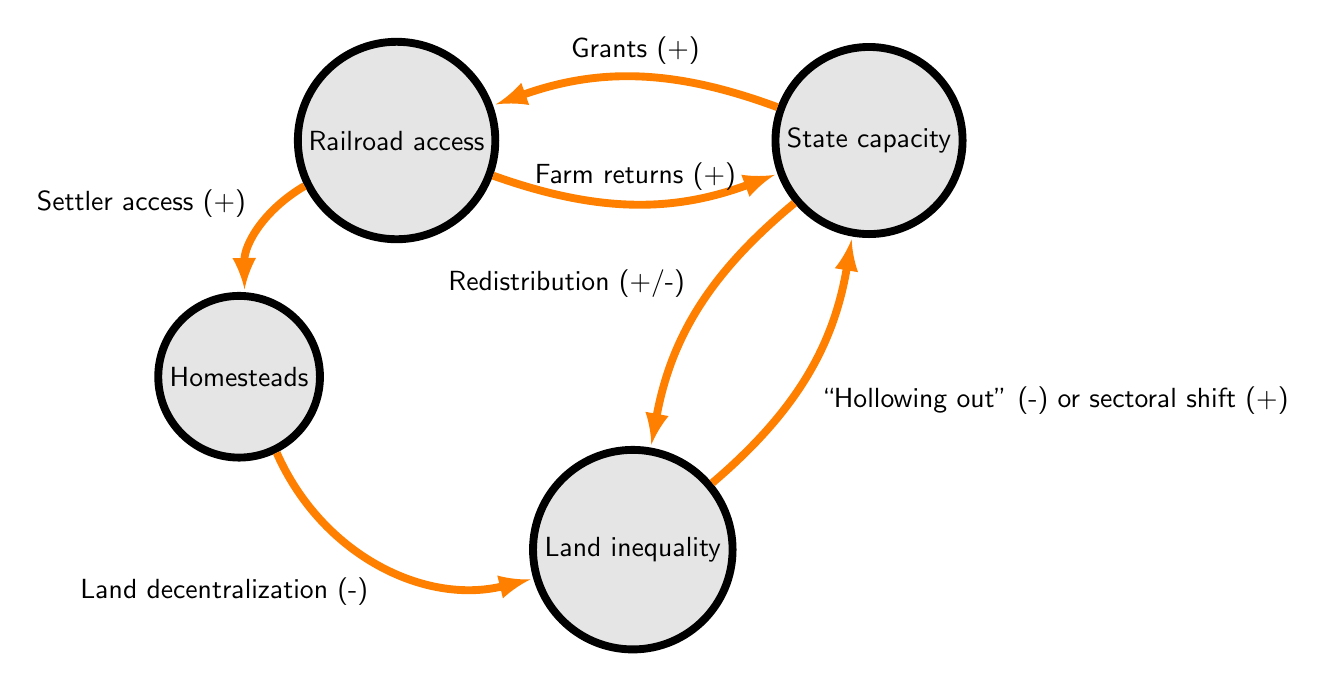
\begin{tikzpicture}[font=\sffamily]
		
		% Setup the style for the states
		\tikzset{node style/.style={state, 
				minimum width=2cm,
				line width=1mm,
				fill=gray!20!white}}
		
		% Draw the states
		\node[node style] at (0, 0)     (railroads)     {Railroad access};
		\node[node style] at (6, 0)     (capacity)     {State capacity};
		\node[node style] at (3, -5.196) (inequality) {Land inequality};
		\node[node style] at (-2, -3) (homesteads) {Homesteads};
		
		% Connect the states with arrows
		\draw[every loop,
		auto=right,
		line width=1mm,
		>=latex,
		draw=orange,
		fill=orange]
		(railroads)     edge[bend right=30]            node {Settler access (+) } (homesteads)
		(railroads)     edge[bend right=20, auto=left] node {Farm returns (+)} (capacity)
		(capacity)     edge[bend right=20]            node {Grants (+) } (railroads)
		(capacity)     edge[bend right=20, auto=center] node {Redistribution (+/-) } (inequality)
		(inequality) edge[bend right=20, auto=center]            node {``Hollowing out'' (-) or sectoral shift (+)} (capacity)
		(homesteads) edge[bend right=40, auto=right] node {Land decentralization (-)} (inequality);
	%	(homesteads) edge[bend right=20, auto=left] node {Demand (+)} (railroads);
		\end{tikzpicture}
\caption{Causal mechanisms underlying the relationship between homesteads and state capacity \label{fig:causal-graph}}
\end{figure}
 % Tables and Figures: introduction
\chapter{Supporting Materials for Chapter \ref{land-reform}}

\begin{figure}[htbp]
	\centering
	\begin{subfigure}[t]{0.48\textwidth}
		\centering
		\includegraphics[width=\textwidth]{/media/jason/Dropbox/github/land-reform/paper/plots/basque_N_16_T_43_numruns_20_num_treated_8_simultaneuous_1.png}
		\caption{Basque Country terrorism data, $N_t = 8$} 
	\end{subfigure}
	~ 
	\begin{subfigure}[t]{0.48\textwidth}
		\centering
		\includegraphics[width=\textwidth]{/media/jason/Dropbox/github/land-reform/paper/plots/california_N_38_T_31_numruns_20_num_treated_19_simultaneuous_1.png}
		\caption{California smoking ban data, $N_t = 19$}
	\end{subfigure}
	~
	\begin{subfigure}[t]{0.48\textwidth}
		\centering
		\includegraphics[width=\textwidth]{/media/jason/Dropbox/github/land-reform/paper/plots/germany_N_16_T_44_numruns_20_num_treated_8_simultaneuous_1.png}
		\caption{West German reunification data, $N_t = 8$} 
	\end{subfigure}
	\caption{Placebo tests under simultaneous treatment adoption. \label{synth-sim}} 
\end{figure}

\begin{figure}[htbp]
	\begin{center}
		\includegraphics[width=\textwidth]{/media/jason/Dropbox/github/land-reform/paper/plots/homestead-heatmap.png}
	\end{center}
	\caption{Per-capita homestead entries in state $i$ and year $t$, 1869-1922. \label{fig:homestead-heatmap}}
\end{figure}

\begin{figure}[htbp]
	\centering
	\begin{subfigure}[t]{0.48\textwidth}
		\centering
		\includegraphics[width=\textwidth]{/media/jason/Dropbox/github/land-reform/paper/plots/exp_pc_N_17_T_159_numruns_20_num_treated_9_simultaneuous_1.png}
		\caption{Expenditures, simultaneous adoption}
	\end{subfigure}
	~ 
	\begin{subfigure}[t]{0.48\textwidth}
		\centering
		\includegraphics[width=\textwidth]{/media/jason/Dropbox/github/land-reform/paper/plots/rev_pc_N_18_T_158_numruns_20_num_treated_9_simultaneuous_1.png}
		\caption{Revenues, simultaneous adoption}
	\end{subfigure}
	~ 
	\begin{subfigure}[t]{0.48\textwidth}
		\centering
		\includegraphics[width=\textwidth]{/media/jason/Dropbox/github/land-reform/paper/plots/exp_pc_N_17_T_159_numruns_20_num_treated_9_simultaneuous_0.png}
		\caption{Expenditures, staggered adoption}
	\end{subfigure}
	~ 
	\begin{subfigure}[t]{0.48\textwidth}
		\centering
		\includegraphics[width=\textwidth]{/media/jason/Dropbox/github/land-reform/paper/plots/rev_pc_N_19_T_158_numruns_20_num_treated_10_simultaneuous_0.png}
		\caption{Revenues, staggered adoption}
	\end{subfigure}
	\caption{Placebo tests under simultaneous and staggered treatment adoption, with $N_t = 9$. \label{mc-sim}} 
\end{figure}

\begin{figure*}[htbp]
	\centering
	\begin{subfigure}[t]{0.43\textwidth}
		\centering
		\includegraphics[width=\textwidth]{/media/jason/Dropbox/github/land-reform/paper/plots/mc-exp-pc-linear.png}
		\caption{Linear interpolation} 
	\end{subfigure}
	~ 
	\begin{subfigure}[t]{0.43\textwidth}
		\centering
		\includegraphics[width=\textwidth]{/media/jason/Dropbox/github/land-reform/paper/plots/mc-exp-pc-median.png}
		\caption{Median replacement}
	\end{subfigure}
	~ 
	\begin{subfigure}[t]{0.43\textwidth}
		\centering
		\includegraphics[width=\textwidth]{/media/jason/Dropbox/github/land-reform/paper/plots/mc-exp-pc-random.png}
		\caption{Random replacement}
	\end{subfigure}
	\caption{MC-NNM estimates of treatment exposure on state government expenditure, using differently imputed data:				
		{\color{Darjeeling15}{\sampleline{}}}, observed treated;
		{\color{Darjeeling11}{\sampleline{dashed}}}, observed control;
		{\color{Darjeeling15}{\sampleline{dotted}}}, counterfactual treated;
		{\color{Darjeeling15}{\sampleline{dash pattern=on .7em off .2em on .05em off .2em}}}, $\hat{\bar{\alpha}}_{t}$.\label{mc-estimates-exp-pc-imp}} 
\end{figure*}

\begin{figure*}[htbp]
	\centering
	\begin{subfigure}[t]{0.43\textwidth}
		\centering
		\includegraphics[width=\textwidth]{/media/jason/Dropbox/github/land-reform/paper/plots/mc-rev-pc-linear.png}
		\caption{Linear interpolation} 
	\end{subfigure}
	~ 
	\begin{subfigure}[t]{0.43\textwidth}
		\centering
		\includegraphics[width=\textwidth]{/media/jason/Dropbox/github/land-reform/paper/plots/mc-rev-pc-median.png}
		\caption{Median replacement}
	\end{subfigure}
	~ 
	\begin{subfigure}[t]{0.43\textwidth}
		\centering
		\includegraphics[width=\textwidth]{/media/jason/Dropbox/github/land-reform/paper/plots/mc-rev-pc-random.png}
		\caption{Random replacement}
	\end{subfigure}
	\caption{MC-NNM estimates of treatment exposure on state government revenue, using differently imputed data:				
		{\color{Darjeeling15}{\sampleline{}}}, observed treated;
		{\color{Darjeeling11}{\sampleline{dashed}}}, observed control;
		{\color{Darjeeling15}{\sampleline{dotted}}}, counterfactual treated;
		{\color{Darjeeling15}{\sampleline{dash pattern=on .7em off .2em on .05em off .2em}}}, $\hat{\bar{\alpha}}_{t}$.\label{mc-estimates-rev-pc-imp}} 
\end{figure*} % Tables and Figures: land-reform
\chapter{Supporting Materials for Chapter \ref{ga-lottery}}

%1
\begin{table}[htbp] 
	\caption{Counties created by 1805 and 1807 lotteries. \label{counties-tab}}
	\begin{tabularx}{\linewidth}{l*{7}{Y}}
		\toprule
		\multicolumn{7}{l}{\textbf{Panel A: 1805}} \\
		\midrule
		Counties  & No. Districts & Lot sizes (acres)& Lot length (chains square)& Lot orientation (degrees) & Grant fee (\$) & Est. value of lot (\$)\\
		\hline
		Baldwin & 5  &  202.5  & 45& 45 / 60  & 8.10  & 839.17\\ 
		Wayne & 3 &  490  &70 &13 / 77  & 19.60 & 842.64 \\ 
		Wilkinson & 5  &  202.5  & 45&45 / 60 & 8.10 & 811.25 \\   
	\end{tabularx}
	\begin{tabularx}{\linewidth}{l*{7}{Y}}
		\toprule
		\multicolumn{7}{l}{\textbf{Panel B: 1807}} \\
		\midrule
		Counties  & No. Districts & Lot sizes (acres)& Lot length (chains square)& Lot orientation (degrees) & Grant fee (\$) & Est. value of lot (\$) \\
		\hline
		Baldwin & 15  &  202.5  & 45& 45 / 60  & 12.15  & 827.35\\ 
		Wilkinson & 23 &  202.5  & 45&45 / 60 & 12.15 & 799.82 \\    
		\bottomrule
	\end{tabularx} 
	\footnotesize{Notes: counties and land lots specified by Acts of 11 May 1803 and 9 June 1806. Lot orientation is degrees from the meridian. Lot values are estimated by averaging the cash value of farms minus the value of farming implements and machinery by the number of (improved and unimproved) acres of land in farms \citep{haines2004,bleakley2013up}. The 1850 values are deflated to 1805 dollars (Panel A) and 1807 dollars (Panel B) using a historical consumer price index \citep{officer2012}.}
\end{table}

%2
\begin{table}[htbp] 
	\begin{center}
		\caption{Distribution of census wealth by officeholding status.}   \label{officeholders-1820-1850}
		\resizebox{1\width}{!}{\input{/media/jason/Dropbox/ga-lottery-local/online-appendix/officeholders-1820-1850}}\\
	\end{center}
	\footnotesize{Notes: slave wealth adjusted to 1850\$ values \citep{williamson2016}. $p$-value is obtained from a Mann-Whitney-Wilcoxon test under the null hypothesis that officeholder and non-officeholder distributions are equal.} 
\end{table}

%9
\begin{table}[htbp]
	\begin{center}
		\caption{Record classification ensemble.\label{ensemble-tab-link}} 
		\begin{tabular}{llcc}
			\hline
			Algorithm & Parameters & MSE & Weight \\ 
			\hline
			\rowcolor{Gray}
			Super Learner & default & 0.02 & - \\
			Generalized boosted regression &  default & 0.02 & 0.05 \\ 
			GLM with elasticnet regularization	 &  $\alpha=0$ & 0.02 & 0 \\  % ridge
			GLM with elasticnet regularization	 &  $\alpha=0.25$ & 0.02& 0 \\ 
			GLM with elasticnet regularization 	&  $\alpha=0.5$ & 0.02 & 0 \\ 
			GLM with elasticnet regularization 	 &  $\alpha=0.75$ & 0.02 & 0 \\ 
			GLM with elasticnet regularization 	 &  $\alpha=1$ & 0.02 & 0.52 \\  % lasso
			Neural network  &  default & 0.13 & 0 \\ 
			Random forests 	& default & 0.02 & 0.32 \\ 
			Random forests 	 & $\# \, \text{variables sampled} =1$ & 0.04 & 0.09 \\ 
			Random forests 	  & $\# \, \text{variables sampled}=5$  & 0.02 & 0 \\ 
			Random forests 	 & $\# \, \text{variables sampled}=10$ & 0.03 & 0 \\ 
			\hline
		\end{tabular} 
	\end{center}
	\footnotesize{Notes: cross-validated risk and weights used for each algorithm in Super Learner prediction ensemble for record classification model. \textit{MSE} is the ten-fold cross-validated mean squared error for each algorithm. \textit{Weight} is the coefficient for the Super Learner, which is estimated using non-negative least squares based on the Lawson-Hanson algorithm. $\alpha$ is the elastic net mixing parameter, where $\alpha = 0$ is the ridge penalty and $\alpha = 1$ is the Lasso penalty. $\# \, \text{variables sampled}$ is the number of predictors sampled for splitting at each node.}
\end{table}

%12
\begin{table}[htbp] 
	\begin{center}
		\caption{Robustness: ITT treatment effects on officeholding.}   \label{officeholding-robust-table}
		\resizebox{0.8\width}{!}{\input{/media/jason/Dropbox/ga-lottery-local/online-appendix/officeholder-robust-table}}
	\end{center}
	\footnotesize{Notes: \textit{Officeholder (match prob.)} is the officeholder match probability. See notes to Table \ref{candidate-robust-table}.}  
\end{table} 

%13
\begin{table}[htbp] 
	\begin{center}
		\caption{Robustness: ITT treatment effects on candidacy.}   \label{candidate-robust-table}
		\resizebox{0.8\width}{!}{\input{/media/jason/Dropbox/ga-lottery-local/online-appendix/candidate-robust-table}}
	\end{center}
	\footnotesize{Notes: \textit{Candidate (match prob.)} is the candidate match probability. Covariates included are those that yield $p <0.10$ in Fig. \ref{balance-plot}.}  
\end{table}  

%14
\begin{table}[htbp] 
	\begin{center}
		\caption{Robustness: ITT treatment effects on slave wealth (1820\$).}   \label{slave-robust-table}
		\resizebox{0.8\width}{!}{\input{/media/jason/Dropbox/ga-lottery-local/online-appendix/slave-robust-table}}
	\end{center}
	\footnotesize{Notes: \textit{Slave wealth (weighted)} is the same measure weighted by the census match probability. See notes to Table \ref{candidate-robust-table}.}  
\end{table}   

\begin{figure}[htbp] %15
	\begin{center}
		\caption{Power analysis by simulation for binary response variable.\label{power-plot-bin}}		
		\includegraphics[width=1\textwidth]{/media/jason/Dropbox/ga-lottery-local/online-appendix/power-plot-bin.png} 
	\end{center}
	\footnotesize{Notes: $N=21,732$ and $\mathcal{I} =100$ iterations. The horizontal line indicates the 80\% power that is normally required to justify a study.}
\end{figure}

\begin{figure}[htbp] % 16
	\begin{center}
		\caption{Quantile regression treatment effect estimates on slave wealth for 1805 winners \& losers. \label{qreg-plot} }
		\includegraphics[width=1\linewidth]{/media/jason/Dropbox/ga-lottery-local/online-appendix/qreg-plot.png} \\
	\end{center}
	\footnotesize{Notes: estimates from a quantile regression of the treatment effect on imputed slave wealth for participants linked to the 1820 Census ($N=5,252$). The points are quantile-specific estimates of the treatment effect and the error bars represent 95\% confidence intervals constructed from bootstrapped standard errors. Quantiles above 0.98 are omitted for display purposes. The line is a LOESS-smoothed estimate of the treatment effect.}
\end{figure}
 % Tables and Figures: ga-lottery
\chapter{Power Analysis by Simulation for Chapter \ref{ga-lottery}}\label{oa-power}

The purpose of a power analysis by simulation is to estimate $\mathrm{P}(\mathrm{Reject \, H_0} | \mathrm{H_0 \, is \, false})$ at a fixed significance level ($\alpha =0.05$) and sample size ($N=21,732$) for different treatment effects $\Delta_{1, \ldots, j}$. In this case $N$ is the size of the observed sample of participants, excluding women and orphans. The simulation proceeds as follows:

\begin{enumerate}
	\item Take a random sample of size $N$ without replacement from from the observed distribution of treatment assignments, weighted by the observed propensity score, to create a vector of simulated treatment assignments.
	\item Simulate response values with $\Delta_{j}$ as the difference-in-means between the simulated treated and control units. Generate random values from the binomial distribution with the probability of success on each trial equal to the mean of the response in the observed sample.
	\item Run linear model on the simulated data and extract the $p$ value.
\end{enumerate}

Repeat the simulation $\mathcal{I}$ times and calculate power of the test by dividing the count of the number of $p$ values that are less than $\alpha$ over $\mathcal{I}$. Normally, 80\% power is required to justify a study.  Fig. \ref{power-plot-bin} provides the results of power analysis simulations for the officeholding response.  % Power analysis by simulation: ga-lottery
\chapter{Supplementary Tables and Figures for Chapter \ref{rnns-causal}}

\begin{figure}[htbp]
	\centering
	\includegraphics[width=0.9\textwidth]{/media/jason/Dropbox/github/rnns-causal/paper/plots/basque-sim.png}
	\caption{Placebo tests on Basque Country terrorism data: 
		{\protect\tikz \protect\draw[color={rgb:red,4;green,0;yellow,1}] (0,0) -- plot[mark=o, mark options={scale=2}] (0.25,0) -- (0.5,0);}, DID;
		{\protect\tikz \protect\draw[color={rgb:red,244;green,226;blue,66}] (0,0) -- plot[mark=triangle*, mark options={scale=2,fill=white}] (0.25,0) -- (0.5,0);}, ED; 
		{\protect\tikz \protect\draw[color={rgb:red,0;green,5;blue,1}] (0,0) -- plot[mark=+, mark options={scale=2}] (0.25,0) -- (0.5,0);}, MC-NNM;
		{\protect\tikz \protect\draw[color={rgb:red,66;green,200;blue,244}] (0,0) -- plot[mark=x, mark options={scale=2}] (0.25,0) -- (0.5,0);}, RVAE;
		{\protect\tikz \protect\draw[color={rgb:red,66;green,107;blue,244}] (0,0) -- plot[mark=diamond, mark options={scale=2}] (0.25,0) -- (0.5,0);}, SCM;
		{\protect\tikz \protect\draw[color={rgb:red,244;pink,66;blue,223}] (0,0) -- plot[mark=triangle, mark options={scale=2, rotate=180}] (0.25,0) -- (0.5,0);}, VT-EN.\label{basque-sim}}
\end{figure}

\begin{figure}[htbp]
	\centering
	\includegraphics[width=0.9\textwidth]{/media/jason/Dropbox/github/rnns-causal/paper/plots/germany-sim.png}
	\caption{Placebo tests on West German reunification data: 
		{\protect\tikz \protect\draw[color={rgb:red,4;green,0;yellow,1}] (0,0) -- plot[mark=o, mark options={scale=2}] (0.25,0) -- (0.5,0);}, DID;
		{\protect\tikz \protect\draw[color={rgb:red,244;green,226;blue,66}] (0,0) -- plot[mark=triangle*, mark options={scale=2,fill=white}] (0.25,0) -- (0.5,0);}, ED; 
		{\protect\tikz \protect\draw[color={rgb:red,0;green,5;blue,1}] (0,0) -- plot[mark=+, mark options={scale=2}] (0.25,0) -- (0.5,0);}, MC-NNM;
		{\protect\tikz \protect\draw[color={rgb:red,66;green,200;blue,244}] (0,0) -- plot[mark=x, mark options={scale=2}] (0.25,0) -- (0.5,0);}, RVAE;
		{\protect\tikz \protect\draw[color={rgb:red,66;green,107;blue,244}] (0,0) -- plot[mark=diamond, mark options={scale=2}] (0.25,0) -- (0.5,0);}, SCM;
		{\protect\tikz \protect\draw[color={rgb:red,244;pink,66;blue,223}] (0,0) -- plot[mark=triangle, mark options={scale=2, rotate=180}] (0.25,0) -- (0.5,0);}, VT-EN.\label{germany-sim}}
\end{figure}

\begin{figure*}[htbp]
	\centering
	\begin{subfigure}[t]{0.48\textwidth}
		\centering
		\includegraphics[width=\textwidth]{/media/jason/Dropbox/github/rnns-causal/paper/plots/educ-dens.png}
		\caption{Unweighted} 
	\end{subfigure}
	~ 
	\begin{subfigure}[t]{0.48\textwidth}
		\centering
		\includegraphics[width=\textwidth]{/media/jason/Dropbox/github/rnns-causal/paper/plots/educ-dens-w.png}
		\caption{Weighted by propensity score}
	\end{subfigure}
	\caption{Pre-period densities of log per-capita state government education spending by treatment status:{\protect\tikz \protect\draw[color=black] (0,0) -- plot[mark=square, mark options={scale=2, fill=white}] (0.25,0) -- (0.5,0);}, Control;
		{\protect\tikz \protect\draw[color={rgb:red,104;green,122;blue,255}] (0,0) -- plot[mark=square*, mark options={scale=2,fill={rgb:red,104;green,122;blue,255}}] (0.25,0) -- (0.5,0);}, Treated \label{educ-dense}} 
\end{figure*}

\begin{figure}[htbp]
	\centering
	\includegraphics[width=0.9\textwidth]{/media/jason/Dropbox/github/rnns-causal/paper/plots/educ-sim.png}
	\caption{Placebo tests on education spending data: 		{\protect\tikz \protect\draw[color={rgb:red,4;green,0;yellow,1}] (0,0) -- plot[mark=o, mark options={scale=2}] (0.25,0) -- (0.5,0);}, DID;
		{\protect\tikz \protect\draw[color={rgb:red,244;green,226;blue,66}] (0,0) -- plot[mark=triangle*, mark options={scale=2,fill=white}] (0.25,0) -- (0.5,0);}, ED; 
		{\protect\tikz \protect\draw[color={rgb:red,0;green,5;blue,1}] (0,0) -- plot[mark=+, mark options={scale=2}] (0.25,0) -- (0.5,0);}, MC-NNM;
		{\protect\tikz \protect\draw[color={rgb:red,66;green,200;blue,244}] (0,0) -- plot[mark=x, mark options={scale=2}] (0.25,0) -- (0.5,0);}, RVAE;
		{\protect\tikz \protect\draw[color={rgb:red,66;green,107;blue,244}] (0,0) -- plot[mark=diamond, mark options={scale=2}] (0.25,0) -- (0.5,0);}, SCM;
		{\protect\tikz \protect\draw[color={rgb:red,244;pink,66;blue,223}] (0,0) -- plot[mark=triangle, mark options={scale=2, rotate=180}] (0.25,0) -- (0.5,0);}, VT-EN.
		\label{educ-sim}}
\end{figure} % Tables and Figures: rnns-causal
\chapter{RNNs Implementation Details for Chapter \ref{rnns-causal}} \label{imp}

The networks are implemented with the \texttt{Keras} neural network library \citep{chollet2015keras} in Python on top of a TensorFlow backend. When implementing encoder-decoder networks, the encoder takes the form of a two-layer Long Short-Term Memory (LSTM) network \citep{schmidhuber1997long}, each with 128 hidden units, and the decoder is a single-layer Gated Recurrent Unit (GRU) \citep{chung2014} also with 128 hidden units. Each recurrent layer uses a linear activation function ($f_1$) with weights initialized using Xavier initialization \citep{glorot2010}. The loss function internally computes the predicted outputs as a linear function ($f_2$) of the log probabilities. 

RNN weights are learned with mini-batch gradient descent on the WMSE using \texttt{Adam} stochastic optimization with the learning rate set to $5\,\cdot\,10^{-4}$ \citep{kingma2014adam}. As a regularization strategy, I apply dropout to the inputs and L2 regularization losses to the network weights. The networks are trained for 1,000 epochs, which takes 10 minutes to run on a laptop CPU. The model is validated on the last 20\% of the training set input-out pairs.  

The RVAE is implemented similarly, but with the following differences: the encoder takes the form of a single-layer LSTM with 32 hidden units and the decoder is a two-layer LSTM with the number of hidden units equal to 32 and the number of predictors, respectively. The latent space $\boldsymbol{z}$ is implemented as a densely-connected layer with a dimension of 200 units and $f_3(\cdot)$ takes the form of a log-normal distribution. The RVAE is trained with stochastic gradient descent for 5,000 epochs, which takes seven minutes to run on the same CPU. % RNNs implementation details: rnns-causal
\chapter{Hypothesis Testing for Chapter \ref{rnns-causal}} \label{eval}

\citet{abadie2010synthetic} propose a randomization inference approach for calculating the exact distribution of placebo effects under the sharp null hypothesis of no effect. \citet{cavallo2013catastrophic} extends the placebo-based testing approach to the case of multiple (placebo) treated units by constructing a distribution of \emph{average} placebo effects under the null hypothesis. \citet{firpo2018synthetic} derive the conditions under which the randomization inference approach is valid from a finite sample perspective and \citet{hahn2017synthetic} analyze the approach from a repeated sampling perspective.

Randomization $p$-values are obtained following these steps:

\begin{enumerate} 
	\item Estimate the observed test static $\boldsymbol{\hat{\upphi}}$ from (\ref{eq:pointwise}). Averaging over the time dimension results in a $\text{T}_\star$-length array of observed average treatment effects. 
	\item Calculate every possible average placebo treated effect $\upmu$ by randomly sampling without replacement which $\text{J}-1$ control units are assumed to be treated. There are $\mathcal{Q} = \sum\limits_{\text{g}=1}^{\text{J}-1} {\text{J} \choose \text{g}}$ possible average placebo effects.\footnote{Since calculating $\mathcal{Q}$ can be computationally burdensome for relatively high values of $J$, I artificially set $\mathcal{Q} = 10,000$ in cases when $\text{J} > 16$.} The result is a matrix of dimension $\mathcal{Q} \times \text{T}_\star$
	\item Sum over the time dimension the number of $\upmu$ that are greater than or equal to $\boldsymbol{\hat{\upphi}}$.  \label{counts}
\end{enumerate}

Each element of the vector obtained from Step \ref{counts} is divided by $\mathcal{Q}$ to estimate a $\text{T}_\star$-length vector of exact two-sided $p$ values, $\hat{p}$. 

\subsection{Randomization confidence intervals}

Under the assumption that treatment has a constant additive effect $\Delta$, I construct an interval estimate for $\Delta$ by inverting the randomization test. Let $\updelta_\Delta$ be the test statistic calculated by subtracting all possible $\upmu$ by $\Delta$. I derive a two-sided randomization confidence interval by collecting all values of $\updelta_\Delta$ that yield $\hat{p}$ values greater than or equal to significance level $\upalpha=0.05$. I find the endpoints of the confidence interval by randomly sampling 500 values of $\Delta$. % Hypothesis testing: rnns-causal

\end{document}
